\documentclass[letterpaper, 11pt]{article}

% Standard packages
\usepackage{amsmath, amsthm, latexsym, amssymb, graphicx, color, mathtools, geometry}

% Simplifies margin settings
\usepackage{geometry}
\geometry{margin=1in,headsep=.25in}

% Puts list item indicators in bold; makes flush with previous margin
\renewcommand\labelenumi{\bf\theenumi.}
\renewcommand\labelenumii{\bf\theenumii.}
\setlength\leftmargini{1.4em}
\setlength\leftmarginii{1.4em}

% Flexibility for headers and footers
\usepackage{fancyhdr}
\usepackage{datetime2}
\usepackage{float}

\pagestyle{fancyplain}
\fancyhf{} %clear all header and footer fields
\cfoot{\bf \small Page \thepage}
\headsep 0.2in
\thispagestyle{empty}

\usepackage[pdftex]{hyperref}
\hypersetup{
    unicode=false,          % non-Latin characters in Acrobat's bookmarks
    pdftoolbar=true,        % show Acrobat's toolbar?
    pdfmenubar=true,        % show Acrobat's menu?
    pdffitwindow=true,      % page fit to window when opened
    pdftitle={My title},    % title
    pdfauthor={Author},     % author
    pdfsubject={Subject},   % subject of the document
    pdfnewwindow=true,      % links in new window
    pdfkeywords={keywords}, % list of keywords
    colorlinks=true,        % false: boxed links; true: colored links
    linkcolor=black,        % color of internal links
    citecolor=green,        % color of links to bibliography
    filecolor=magenta,      % color of file links
    urlcolor=blue           % color of external links
}

\renewcommand{\headrulewidth}{0pt}

\parindent 0in
\parskip 12pt

\begin{document}

\title{Homework Template}

\begin{center}
    {
        \large
        \bf
        CS-E4850 Computer Vision\\
        Exercise Round \#12\\
        Submitted by Chen\ Xu, ID 000000\\
        \today
    }
\end{center}
\bigskip
\textbf{Exercise 1. Course feedback.}\\
\textbf{Exercise 2. Epipolar geometry.}


\begin{figure}[H]
    \centering
    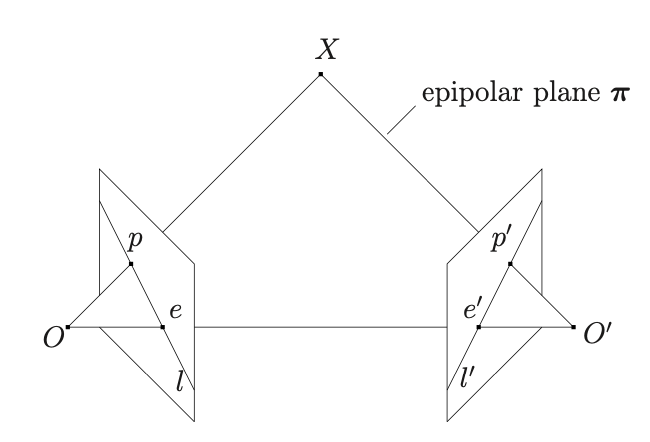
\includegraphics[width=0.6\columnwidth]{EpipolarGeometry.png}
    \caption{Epipolar geometry}
    \label{fig:epi_geo}
\end{figure}

\begin{proof}
    \begin{align}
        \overrightarrow{O'p'}\cdot(\overrightarrow{O'O}\times\overrightarrow{Op})            & =0          \\
        \Rightarrow \textbf{x}'\cdot(\textbf{t}\times(\textbf{R}\textbf{x}+\textbf{t}))      & =0\nonumber \\
        \textbf{x}'\cdot(\textbf{t}\times(\textbf{R}\textbf{x})+\textbf{t}\times\textbf{t})) & =0\nonumber \\
        \textbf{x}'\cdot(\textbf{t}\times(\textbf{R}\textbf{x}))                             & =0\nonumber \\
        \textbf{x}'^\top[\textbf{t}]_\times\textbf{R}\textbf{x}                              & =0\nonumber \\
        \Rightarrow\textbf{x}'^\top\textbf{E}\textbf{x}                                      & =0\nonumber
    \end{align}
    where $\textbf{E} = [\textbf{t}]_\times\textbf{R}$
\end{proof}
\newpage
\textbf{Exercise 3. Stereo vision.}
\begin{figure}[H]
    \centering
    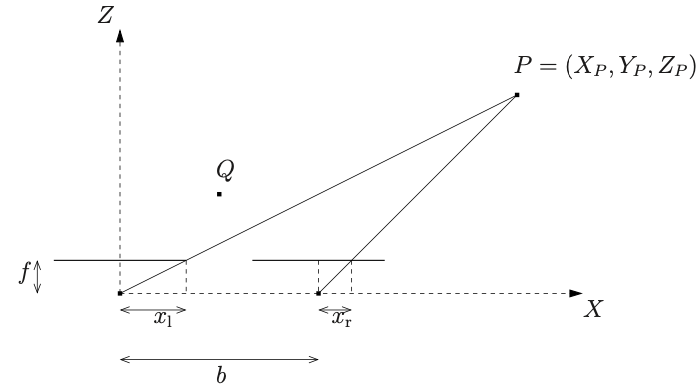
\includegraphics[width=0.6\columnwidth]{Stereo.png}
    \caption{Stereo vision}
    \label{fig:ste_vis}
\end{figure}
a)
$$
    Z_p = \frac{b}{d}f = 6\ cm
$$

b)
$$
    \Delta Z = \frac{b}{\Delta d} f = 60\ m
$$

c)
\begin{align*}
    \textbf{x}_l^Q & = \textbf{P}_l \textbf{X}^Q \\
    \textbf{x}_l^Q & =
    \begin{bmatrix}
        1 & 0 & 0 & 0 \\
        0 & 1 & 0 & 0 \\
        0 & 0 & 1 & 0
    \end{bmatrix}
    \begin{bmatrix}
        3 \\
        0 \\
        3 \\
        1
    \end{bmatrix}                               \\
                   & =
    \begin{bmatrix}
        3 \\
        0 \\
        3
    \end{bmatrix}                               \\
                   & =
    3
    \begin{bmatrix}
        1 \\
        0 \\
        1
    \end{bmatrix}
    \intertext{So the in-homogeneous coordinate of Q on the image plane of the camera on the left is}
    \textbf{x}_l^Q & =
    \begin{bmatrix}
        1 \\
        0
    \end{bmatrix}
\end{align*}

From the Epipolar constraint:
$$ \textbf{x}'^\top\textbf{E}\textbf{x}=0 \text{,\ } \textbf{E} = [\textbf{t}]_\times\textbf{R}$$
$$ \textbf{R} = \textbf{I}$$
\begin{align*}
    \textbf{t} & = (T, 0, 0) = (-6, 0, 0)       \\
    \therefore
    \textbf{E} & =[\textbf{t}]_\times\textbf{R} \\
               & =
    \begin{bmatrix}
        0 & 0  & 0 \\
        0 & 0  & 6 \\
        0 & -6 & 0
    \end{bmatrix}                              \\
\end{align*}
\begin{align*}
    \begin{pmatrix}
        u' & v' & 1
    \end{pmatrix}
    \begin{bmatrix}
        0 & 0  & 0 \\
        0 & 0  & 6 \\
        0 & -6 & 0
    \end{bmatrix}
    \begin{pmatrix}
        u \\
        v \\
        1
    \end{pmatrix}
              & =0                                                                               \\
    \begin{pmatrix}
        u' & v' & 1
    \end{pmatrix}
    \begin{pmatrix}
        0 \\
        6 \\
        -6v
    \end{pmatrix}
              & =0                                                                               \\
    6 v' -6 v & =0                                                                               \\
    v' = v    & = 0                                                                              \\
    \intertext{The corresponding epipolar line on the image plane of the camera on the right is} \\
    v'=0      &     &
\end{align*}

\textbf{Exercise 4. Fundamental matrix estimation.}

\end{document}
